\section{Sensibility Testbed Architecture}\label{sec-design}

The architecture of Sensibility Testbed is comprised of three main components that are critical 
to its operation, as shown in Figure~\ref{fig-arch}. In this section, we discuss each of these components in 
greater detail, describing their functions and introducing several key 
techniques that make the testbed's enhanced security possible. 

\subsection{Device Software}\label{sec-repy}

%In Sensibility Testbed, all experiments execute in a secure 
%sandbox on the end devices.
%Experimenters' code executes in a sandbox that isolates the 
%experiment code from the device host system. 
The device software of Sensibility Testbed is the only one of the three 
components that runs on end users' devices. It is divided into three 
parts: a secure sandbox called Repy (Restricted Python), a resource 
manager that facilitates the interaction between researchers and the 
sandbox, and a device manager that allows the device owner to control 
if the sandbox and resource manager can run on the device.


\subsubsection{Secure Sandbox} 
The Repy sandbox is the most important in the device software. This 
security-reviewed sandbox~\cite{cappos2010retaining} mitigates the 
impact of bugs in experimenter code by providing security isolation 
and performance isolation\footnote{\scriptsize 
This sandbox has been used successfully for more than six years in our 
prior work, the Seattle testbed~\cite{seattle}.}. 
%Instead of developing full-fledged Android apps, all 
%experiments in Sensibility Testbed are written in a language
%similar to Python, and run in a secure %Python-based
Researchers use a Python-like programming interface~\cite{repyv2}
to write experiment code, upload the code and execute it in the
sandbox on remote devices. The programming interface includes functions for networking, 
file system access, threading, locking, logging, and so on. To access sensors, 
the sandbox also has a set of sensor functions~\cite{sensors}. 
%Details about implementing the Repy sandbox for mobile 
%devices are described in Section~\ref{sec-repy-ext}.
%
%However, the current Repy sandbox does not include calls to access sensors. 
%%To obtain the sensor data, we need to extend the sandbox. 
%The extended Repy sandbox that allows sensor access  
%will be described in Section~\ref{sec-repy-ext}.
Another important feature of the Repy sandbox allows us to change the 
behavior of its programming interface, and control the 
data gathered from the device to adapt to any IRB proscribed limits. 
%For  an experiment
%that involves GPS location, a privacy policy might restrict the
%level of data granularity available to the experiment. For example, it can
%obfuscate GPS location such that it only identifies the center
%of the city that the device is located in, rather than the exact
%location. Using the same technique, 
For example, the sandbox can anonymize the IP address of a device, constrain  
the frequency of access to GPS locations, and disable
access to cameras. 
%Such privacy protection is a contribution of Sensibility Testbed, 
%which does not exist in any prior work. 
The details of policy implementation are presented in 
Section~\ref{sec-layer} and \ref{sec-nanny}.

\textbf{Security and performance isolation.}
The sandbox is the execution environment 
of all experiment code. It isolates experimenters' programs from one 
another, and prevents any of the code from harming the device 
through its strong isolation techniques. More importantly, the sandbox
provides a flexible system call interposition technique where system call behavior 
can be modified. This allows us to define and implement
different data access policies. 

Repy has a small, self-contained kernel as its trusted 
computing base (TCB). %unprivileged libraries and experiment code. 
Every system call in the TCB is strictly 
sanitized to preserve consistent behavior across different OSes, 
and to avoid uncommon corner cases that can be exploited. 
Furthermore, since the TCB is small (about 8,000 lines of code), it is 
less likely to have a kernel exploit than other more complex kernels. 
As a result, any vulnerability in an experiment 
%can at most cause compromise in the unprivileged portion of the sandbox, 
cannot escape the sandbox and perform malicious actions to 
the device system. The Repy sandbox exposes its system calls for 
accessing resources on a device through a Python-like programming 
interface~\cite{repyv2} isolating experiment code from the kernel. 
%another way of saying this:
%Experiment code for accessing resources is contained by the 
%Repy sandbox, using its Python-like programming language interface.
This same sandbox design has been successfully running experiments as part of a network research 
testbed for more than six years, without significant operation faults or security breaches~\cite{seattle}. \yanyan{Justin thinks this statement is weak.} \lois{I don't know if this answers his concerns since the meaning is essentially the same}
%=======
%through a Python-like programming interface~\cite{repyv2}. 
%%to experiment code for accessing resources on a device. 
%%another way of saying this:
%%Experiment code for accessing resources is contained by the 
%%Repy sandbox, using its Python-like programming language interface.
%This same sandbox design has been successfully running experiments 
%as part of a network research testbed~\cite{seattle} for more than six 
%years, with no report of operational faults or security breaches. 
%>>>>>>> yyzhuang/master

In addition to security isolation,
%The sandbox exposes a programming 
%interface to experimenter programs to access 
%resources on the device. 
the sandbox provides performance isolation by
%by using OS hooks to monitor and control the amount of 
%CPU and memory used by a sandboxed program. To restrict 
%other resources, such as network and disk I/O, the sandbox 
interposition on system calls~\cite{garfinkel2003traps} that 
use resources, such as network and disk I/O, and preventing 
or delaying the execution of these calls if they exceed 
their configured quota. 
%As a result, this sandbox limits 
%what a sandboxed program can do. For example, 
This isolation means the sandbox can set access limits. For example, 
reading from and writing to the file system can
only occur in a per-experiment directory, sending and receiving
data via the network interface cannot exceed a configured rate, and 
CPU, memory and battery consumption cannot exceed a set level.
Therefore, the sandbox isolates the experiment program from 
the rest of the device. Due to this isolation, different researchers 
can run experiments on different sandboxes on the same device, 
without any interference between the experiments.

\begin{figure}
\center{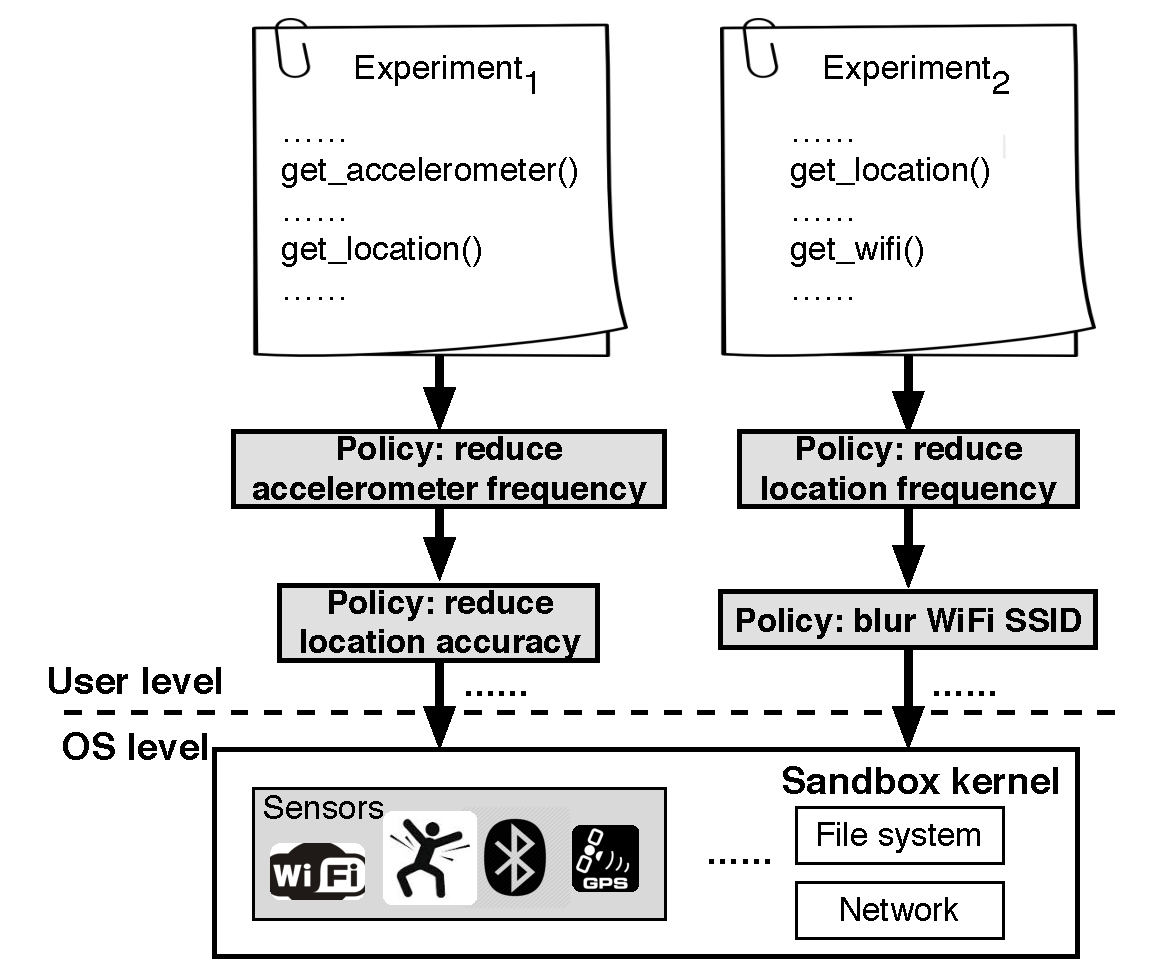
\includegraphics[width=0.9\columnwidth]{figs/blur.pdf}}
%\vspace*{-20pt}
\caption{\small Policy stack demonstrating how Sensibility Testbed implements blur policies.
\label{fig-blur}}
\end{figure}

\textbf{Policy stack.}
In Sensibility Testbed, privacy policies are implemented as blurring layers, with each layer acting as a 
reference monitor in the sandbox~\cite{ref} to enforce an access 
control policy over each sensor. Using the sandboxing 
technique in our prior work~\cite{cappos2010retaining}, we are able to
interject code to control the behavior of sandbox functions, or 
system calls. A sensor access policy can (1) reduce 
the precision of the raw sensor data returned from a device, such
as returning the location of a nearest city rather than the device's exact location, and (2) restrict 
the frequency of access to a sensor, such as the polling rate of a gyroscope or
an accelerometer, to avoid password interference~\cite{michalevsky2014gyrophone}.

%and (3) disable  
%access to a certain sensor in sensitive situations, such as 
%turning off a camera when a device is in a residential or work area.
%Implementation of the last policy is still ongoing, so this paper will mainly address
%how blurring layers allow for the execution of the first two types of policies. 

%The sandbox kernel determines how IRB policies are implemented by affecting system calls. It can
%interpose on a call and modify the data returned, or control the frequency with which a call can be made over
%a period of time. 

%Different policies implemented can be stacked in tandem to 
%control different sensor accesses, like in Figure~\ref{fig-blur}.
%As mentioned above, Bob provided his IRB policies through our clearinghouse.
%Before Bob runs his experiment, the clearinghouse loads the access policies and instructs the sandbox on Alice's device to
%restrict sensor access accordingly. 
%
%Using the \path{get_location()} call as an example, 
%when Bob's code requests location data from Alice's device, the Repy sandbox first
%invokes the location-related Android code. 
%%(line 10 in Figure~\ref{fig-getlocation}). 
%When the location data is returned, according to Bob's IRB policy
%indicates that the returned location coordinates should be blurred to the nearest city to Alice's
%device, instead of her actual location. As a result, 
%For example, the sandbox returns a perturbed location that is less accurate, 
%%Furthermore, as Bob's IRB policy disallows collecting information about cell tower IDs, 
%%blocks any access to cell IDs, 
%%by another policy. Similarly, other information
%blurs a WiFi SSID to a hashed string, and restricts the frequency to access a
%gyroscope to prevent inferring passwords~\cite{michalevsky2014gyrophone}, and so on. 
Each policy is a blurring layer, which defines either of the above
two categories of policies. Different sets of policies can be customized 
according to the regulations set by IRB, through loading 
individual blurring layers in order, as a policy stack. In each stack, 
a lower layer is the ancestor of a higher layer. Every layer inherits 
the policy defined by its ancestor layers, with the exception of the lowest layer. 
%Each blurring layer is untrusted by its ancestor layers, 
%but is trusted by its descendant layers. \yanyan{maybe cut this.}
The lowest blurring layer with no ancestors is the 
Sensibility Testbed's sandbox kernel. The experiment program runs at the top 
of the policy stack, thereby inheriting all the policies defined by the
lower layers, as shown in Figure~\ref{fig-blur}. 
Each policy stack acts as a set of filters for different sensors, through 
which a call must pass before a sandboxed program can
access the sensor data. 
%Different stacks can be customized for different IRB policies.


%In the following, we describe how to implement each blurring layer, 
%and use them to form a policy stack.

\textbf{Data precision and data access frequency.}
\yanyan{I feel this may better be placed in implementation section.}
Reducing data precision partially protects a device owner's privacy. However, frequent data 
access can be another channel to snoop on personal information.
If sensor queries are made on a sufficiently frequent basis, they can be used
to track an individual's activity. The goal of reducing sensor access frequency 
is to prevent an accumulation of identifiable information, such as 
location~\cite{gruteser2003anonymous}, wireless network identifiers, and even 
accelerometer data. (Note that specific
details as to how frequently a certain sensor can be accessed without risking such an 
invasion is out of the scope of this work). 
Furthermore, the battery power of a device can 
be drained faster if sensors are accessed
with unnecessary frequency. Therefore, restricting the data access rate 
mandates that experiments collect data only as often as is necessary. 
To achieve this, the Repy sandbox provides a second mechanism
called \path{nanny} that mediates and restricts access frequency to sensors. 

\path{nanny} treats all sensors as \textit{resources}, and the function calls to 
access the sensors as the \textit{usage} of resources. 
%\path{nanny}'s control 
%mechanism for a resource is to limit the \textit{rate} of its usage. For example, 
When an 
%Utilization is controlled over one or more periods, where
experiment program's use of a resource is above a given threshold, 
\path{nanny} pauses the 
program for as long as required to bound it, on average, below the
threshold. Therefore, if an experiment program attempts to 
use a resource at a rate faster than is allowed by a policy, the function 
call is blocked until sufficient time has passed to average out the overall access rate. 
To monitor and control the usage of resources, \path{nanny} keeps a 
table of resource assignments that tracks and updates requests and releases. 
Once resource caps are set, an experiment program can never call a 
function to access a sensor more frequently than the cap. 


\subsubsection{Resource Manager} The second part of the device software, called a resource manager, 
establishes a trust relationship between a device and a researcher. It 
manages a researcher's access to the sandboxes on a device, and
controls the start and stop of the sandboxes on the device. The 
resource manager controls which researchers can access the 
sandbox on any given device, and communicates with the clearinghouse
or experiment manager. If multiple researchers have access to 
the same device, the resource manager splits the resources in the 
sandbox among the researchers, and partitions the one sandbox 
into several smaller ones. In order for the clearinghouse or a 
researcher's experiment manager to discover the sandbox on a 
device, the resource manager also contacts a lookup service that 
announces the existence of the available devices. An example is 
given in Section~\ref{sec-case1}.

\subsubsection{Device Manager} The last part of the device software is a device manager that 
allows device owners to manage the software running on their 
devices. This is the only part of device software that a device owner 
will interact with directly. With the device manager, a device owner  
can install and remove the device software, and start and stop the 
operations. The device manager also provides a user interface to 
allow a device owner to opt out of any experiment. Thus, the device 
owner has the freedom to choose what experiments will be allowed 
to run on the phone or tablet.


\subsection{Clearinghouse}\label{sec-ch}
The clearinghouse~\cite{ch} is a testbed server that has two 
responsibilities. First, it keeps track of devices and grants 
researchers access to available devices; and second, it
sets up the relevant IRB policies for each individual experiment that 
must be enforced through the sandboxes on remote devices.
%It allows experimenters to register accounts and share 
%access to a common pool of devices.
Researchers register their experiments at the clearinghouse, and 
provide their institution's IRB 
policies. When an account is approved, the researcher is assigned 
a pair of public/private \textit{authentication keys} by the 
clearinghouse, to authenticate himself with the clearinghouse. This
researcher can then sign into his account and request a 
number of sandboxes for his experiment. The clearinghouse 
looks up available sandboxes on behalf of the researcher by 
querying the lookup service. Once a sandbox is discovered, the 
clearinghouse stores the sandbox's meta information, 
%\textit{identification key}, 
and assigns it to the researcher's experiment account. 

Besides assigning devices, the clearinghouse also has the role of 
instructing the sandboxes assigned to this researcher to add the IRB 
policies specified during registration. The clearinghouse does so 
by communicating with the resource managers on those devices, which 
control the code executed in the sandboxes. The involvement of the 
clearinghouse in any given experiment ends 
after the researcher deploys his code to the devices. It does not store any
data on the researcher's behalf. 
This Sensibility Testbed clearinghouse 
protocol for research with device owners has been approved by
the IRB at New York University (IRB \# 15-10751). An example 
of this protocol in operation is given in Section~\ref{sec-case2}.

%However, it can direct the release of data to a server designated by the 
%researcher. To do so, the experimenter must register
%his server by providing its certificate and URL to the
%clearinghouse, which will then instruct the devices
%accessible to the experimenter that all the sensor data collected should be
%sent to this server. The sandboxes on these devices will issue
%\texttt{HTTPS POST} using the server's certificate, and send encrypted
%data to the experimenter's server.

%The key role of this component is to facilitate device sharing, 
%which relieves individual experimenters from repeatedly 
%recruiting devices for each experiment.
%
%Note that in Sensibility Testbed, there are two types of keys. A device
%owner has an \textit{identification key} to identify the app installed on a 
%device. This key is mostly used by a lookup service. 

%This pair of keys are mostly used by the clearinghouse and 
%experiment manager.

%\lois{have you introduced the idea of keys yet? If not, I think this needs to be explained.}


\subsection{Experiment Manager}\label{sec-emt}

The last component in the testbed is an experiment manager, which a 
researcher can download to his own computer and use to run code in 
%which contains Bob's private key, \path{key.bob-priv}, 
the sandboxes on the remote devices. 
The researcher uses the experiment manager as a light-weight command line 
console~\cite{demo-kit} to directly access the remote devices, upload 
experiment code written in the Repy programming interface, and
communicate with the resource manager on the device to start 
or stop the execution of the experiment. To authenticate himself with 
the remote sandbox, the researcher uses 
his public/private key pairs to establish a secure connection from his
computer. The experiment manager can also be used to download data 
from the remote devices to the researcher's local computer, or
the researcher can set up his own server to store the data\footnote{\scriptsize
If an experimenter stores data on his own server, he must use protective
measures to ensure that data sent from the mobile devices is
properly encrypted, and the server storage cannot be tampered
with by any other parties. This is enforced by requiring the experimenter to register
his server by providing its certificate and URL to our
clearinghouse. Following receipt of this data, the clearinghouse will instruct the devices
accessible to the experimenter that all the sensor data collected should be
sent to this server. The sandboxes on these devices will issue
\texttt{HTTPS POST} using the server's certificate, and send encrypted
data to the experimenter's server.}. 
If an experimenter stores data on his own server, he must use protective
measures to ensure that data sent from the mobile devices is
properly encrypted, and the server storage cannot be tampered
with by any other parties. Researchers can also opt to use a data 
store service we provide (a service called Sensevis~\cite{sensevis}, 
not shown in Figure~\ref{fig-arch}). After the data is collected, the method of 
securely storing the data will be mandated by the researcher's IRB.

\smallskip
This Sensibility Testbed clearinghouse protocol for research plays a central role in
easing the process of device recruitment and experiment setup for experimenters, 
and ensures the enforcement of privacy policies. 
%Prior to running an experiment on Sensibility Testbed, a
%experimenter first fills out a form in plain text to describe the
%purpose of the research experiment. This experiment description
%is created at the Sensibility Testbed clearinghouse
%where the researcher indicates the type of data to be collected,
%how that data will be used and stored, and so on. 
%
%Once this information is collected from the researcher, the
%clearinghouse automatically generates a set of blurring layers
%that implements the experiment policy (Section~\ref{sec-policy}). In
%Sensibility Testbed, researchers can collect data from the
%sensors on the device, such as GPS, Bluetooth, battery
%information, accelerometer, light, and orientation,
%etc. The blurring layers we provide consist of
%data access restrictions, created in accordance with
%researcher's experiment description, by using the Sensibility
%Testbed's sandboxing technique 
%(Section~\ref{sec-repy})~\cite{cappos2010retaining}. These restrictions ensure that
%the researcher cannot conduct experiments to access data that
%extend beyond the experiment policy. 
%
%This Sensibility Testbed
%clearinghouse protocol for research plays a central role in
%easing the approval process of IRB, and ensures the enforcement
%of privacy policy\footnote{The Sensibility Testbed Clearinghouse
%protocol for research with human subjects has been approved by
%the IRB at New York University. \yanyan{might need a link to
%your approval letter or ref number}}. 
Using Sensibility Testbed, device owners' privacy is protected
from any inadvertent or malicious attempt, and researchers 
are able to go through a streamlined process of device 
recruitment and experiment setup.

